\chapter{La machine à courant continu}
Ces machines ne sont plus utilisées comme génératrices de puissances 
mais leurs capacité de réglage de vitesse nous pousse à les étudier. 
\textbf{Dynamo} est le nom donné à une génératrice à courant continu.

\section{Génération d'une tension continue}
	\subsection{Effet d'un collecteur}
	Pour avoir une f.e.m. continue, il faut 
	\begin{enumerate}
	\item Un collecteur
	\item Augmenter le nombre de conducteurs actifs
	\end{enumerate}
	Le \textbf{collecteur} est un commutateur ayant pour but de 
	redresser la f.e.m. alternative\footnote{"En électrotechnique, 
	un collecteur commutateur rotatif est un organe permettant de 
	créer 	une connexion électrique entre une partie fixe (stator) 
	et une 	partie tournante (rotor), avec une fonction de 
	commutation pendant la rotation. On trouve ce genre de 
	collecteur dans les machines à courant continu et les moteurs 
	électriques universels.".}.\\
	\begin{wrapfigure}[10]{l}{8.2cm}
	\vspace{-5mm}
	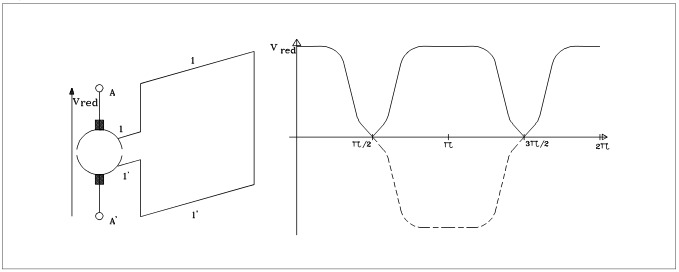
\includegraphics[scale=0.34]{ch4/image1.png}
	\captionof{figure}{ }
	\end{wrapfigure}
	\textbf{Petit plus (Source : Wikipedia) :} \textit{Ce collecteur 
	commutateur rotatif consiste en un anneau conducteur de l'électricité  
	sectionné en un nombre pair de parties 
	isolées entre elles, fixé avec une entretoise isolante sur l'axe de 
	la machine. La connexion électrique est créée entre les parties 
	conductrices et la partie fixée sur le stator (bornier), par une ou 
	plusieurs paires de balais positionnées respectivement à 180$\ ^\circ$. 
	On alimente en électricité le bobinage du rotor par ces contacts 
	(fonctionnement en moteur) ou au contraire on récupère l'électricité 
	produite par le bobinage du rotor (fonctionnement en générateur).}\ \\
	
	L'idée de l'espacement de $\pi$ est que le sens du courant dans 
	l'anneau conducteur va s'inverser, permettant au rotor de continuer 
	à tourner comme on peut le voir sur l'illustration ci-contre.\\
	On obtiendra aux balais une f.e.m. unidirectionnelle et dans le circuit 
	extérieur un courant unidirectionnel. Cependant, la grandeur ce cette 
	f.e.m. et du courant qui en résulte ne sont pas constantes.
	
	\newpage
	\begin{wrapfigure}[11]{r}{6.8cm}
	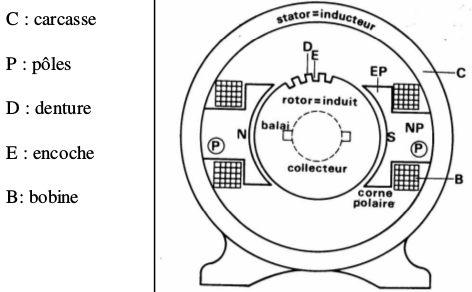
\includegraphics[scale=0.4]{ch4/image2.png}
	\captionof{figure}{ }
	\end{wrapfigure}
	Considérons un exemple "réel". Cette machine est constituée de 
	\begin{itemize}
	\item[$\bullet$] Un inducteur, sur le stator possédant $p$ paires de 
	pôles saillants. La répartition de l'induction dans l'entrefer a une 
	forme trapézoïdale avec comme axe de symétrie l'axe \textit{longitudinal} 
	$d$. L'axe électriquement $\perp$ à celui-ci est l'axe \textit{transversal},
	$q$.
	\item[$\bullet$] 	Un induit, disposés sous la forme d'enroulements de 
	conducteurs placés dans les encoches du cylindre rotorique. On connecte 
	via les faces latérales du cylindre ces conducteurs pour former un 
	\textit{enroulement en tambour.} 
	\end{itemize}\ 
	
	Les conducteurs actifs réunis par ces liaisons sont situés sous les 
	pôles opposés, d’où il résulte une addition des f.e.m. induites.
	Le point médian de chaque conducteur est relié à une lame du collecteur. 
	La \textbf{commutation} d’une lame à l’autre se fait donc au moment 
	où un conducteur actif passe d’un pôle à l’autre. Il faut voir que la somme des 
	f.e.m est nulle dans toute la machine, ce n'est qu'au niveau des ballais où on 
	somme d'une part toutes les f.e.m positives et sur l'autre les négatives. Ces 
	groupes de conducteurs actifs sont appelé \textbf{dérivations}.
	
	
	\subsection{Machine multipolaire}
	\begin{wrapfigure}[8]{l}{4.5cm}
	\vspace{-5mm}
	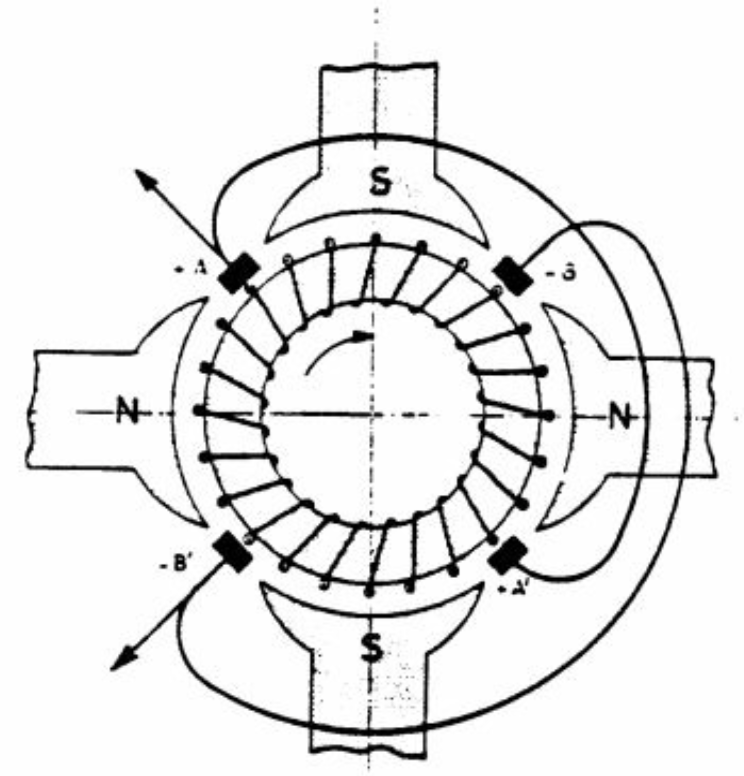
\includegraphics[scale=0.3]{ch4/image2p.png}
	\captionof{figure}{ }
	\end{wrapfigure}
	On considérait jusqu'ici des machines à deux pôles inducteurs, soyons 
	fous et plaçons-en maintenant quatre. Par symétries, les f.e.m. seront 
	égales en grandeurs puisqu'on somme une tension soit positive soit négative 
	entre deux ballais\footnote{Enes se représente la situation du sens des courants en utilisant $q\vec{v}\times \vec{B}$ qui donne des courants entrant aux pôles N et des courants sortant aux pôles S. Sachant que $v = \frac{d\phi}{dt} = \frac{d}{dt}\int \vec{B} \vec{dS}$ et que la convention d'Haelterman disait que le $\vec{dS}$ est donné par la règle de la main droite quand on tourne avec le courant, on peut voir que le produit scalaire de B et dS est positif avant les ballais + et négatif avant les ballais -. C'est comme ça qu'il expliquerai la sélection des ballais positif et négatif.}. Si l'on connecte les balais opposés entre eux (
	les deux négatifs ensemble, de même pour les positifs) on obtient une 
	dynamo multipolaire à \textit{enroulement parallèles}. \\\\\\
	
	\subsection{Types d'enroulement d'induit}
	Problème complexe non abordé ici. Sachez juste que pour l'enroulement 
	en tambour, on peut avoir l'enroulement \textit{imbriqué} ou l'
	enroulement \textit{ondulé}.
	
	\subsection{Tension à vide en régime statique}
	Soit un enroulement en tambour (l'armature, $a$) de $N_C$ conducteurs 
	répartis uniformément en deux couches. Le nombre de spires $N_S=N_C/2$. 
	On va supposer l'induit infiniment divisé de sorte à avoir une densité 
	linéique de spires $N_S/(2\pi R)$. On suppose un rotor lisse.
	
		\subsubsection{Méthode des champs}
		\begin{wrapfigure}[11]{l}{4.8cm}
		\vspace{-5mm}
		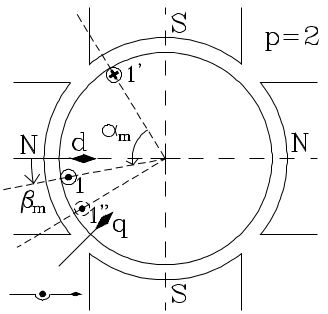
\includegraphics[scale=0.4]{ch4/image3.png}
		\captionof{figure}{ }
		\end{wrapfigure}
		Soit une spire constituée d'un conducteur d'entrée 1 et de sortie 
		1'. Nous avons
		\begin{description}
		\item[$\beta_m$ :] la coordonnée angulaire mécanique de l'entrée 1
		\item[$\beta_m-\alpha_m$ :] la coordonnée mécanique de sortie 1'
		\end{description}				
		La f.e.m. engendrée dans la spire vaut (voir figure ci-contre pour 
		la convention de signe (conducteur entrant et sortant))
		\begin{equation}
		\begin{array}{ll}
		e_{spire} &= B(\beta_m)lv - B(\beta_m-\alpha_m)lv\\
		&= (B(\beta_m)-B(\beta_m-\alpha_m))lv
		\end{array}
		\end{equation}
		Si $\alpha_m = \pi/p$ la spire est \textit{diamétrale}. Le "sens" 
		du champ $B$ sera donc exactement opposé
		\begin{equation}
		\begin{array}{l}
		B(\beta_m-\alpha_m) = - B(\beta_m)\\
		\hookrightarrow e_{spire} = 2B(\beta_m)lv
		\end{array}
		\end{equation}
		Si $\alpha_m<\pi/p$ on parle de spire \textit{à pas raccourci} : 
		on définit 1" déphasé de $\pi/p$ en avant par rapport à 1' et 
		donc déphasé de $\delta_m = \pi/p-\alpha_m$ par rapport à 1. Par 
		symétrie\footnote{??}
		\begin{equation}
		 \begin{array}{ll}
		B(1') = -B(1")\qquad\text{ou}\qquad B(\beta_m-\alpha_m) &=-B(\beta_m
		-\alpha_m+\frac{\pi}{p})\\
		&=-B(\beta_m+\delta_m)		
		\end{array}
		\end{equation}
		Impliquant que $e_{spire} = e_1-e_{1'}=e_1+e_{1"}$, en considérant 
		$B>0$ sous la pôle nord.\\
		On peut alors avoir une répartition rectangulaire de l'induction
		\begin{center}
		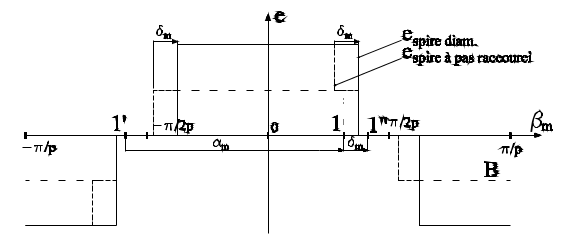
\includegraphics[scale=0.5]{ch4/image4}
		\end{center}
		ou  trapézoïdale 
		\begin{center}
		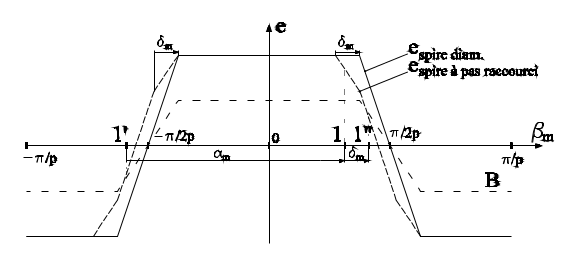
\includegraphics[scale=0.5]{ch4/image5}
		\end{center}
		
		\textsc{Forces électromotrice entre balais}\ \\
		\begin{wrapfigure}[12]{l}{6cm}
		\vspace{-2mm}
		\begin{equation}
		\begin{array}{ll}
		e &= \displaystyle p \int_{-\frac{\pi}{2p}}^{\frac{\pi}{2p}} 
		e_{spire}.\text{densité de spire}\\
		&= \displaystyle p \int_{-\frac{\pi}{2p}}^{\frac{\pi}{2p}} (
		2B(\beta_m)kv)\frac{N_s}{2d\pi}\ d\beta_m\\
		&= \displaystyle \frac{p}{d}N_s\frac{\Omega_r}{\pi} \int_{-
		\frac{\pi}{2p}}^{\frac{\pi}{2p}}B(\beta_m)lR\ d\beta_m\\
		&= \displaystyle\frac{p}{d}N_s\frac{\Omega_r}{\pi}\Phi
		\end{array}
		\end{equation}

		\end{wrapfigure}
		Supposons un enroulement à spires diamétrales tel que $e_{spire} = 
		2B(\beta_m)lv$. La f.e.m. entre balais est constante si l'induit 
		est infiniment divisé. Considérons un enroulement ondulé à $2d$ 
		dérivations : une dérivation comporte $N_S/(2d)$ spires. Celle-ci 
		est constitués par des spires dont les conducteurs d'entrée et 
		de sorties sont sous des pôles de même signe, il y a donc 
		$(N_S/2d).(1/\pi)$ spires appartenant à une dérivation par rad. 
		mécanique. Pour obtenir la tension aux bornes de la dérivation, 
		il faut intégrer les tensions de chaque spire de la dérivation. 
		Comme il y a $p$ paires de pôles, il convient de multiplier le 
		résultat d'un pôle par $p$. De façon générale :\\
		
		\retenir{\begin{equation}
		e = K\ \Omega_r\ \Phi
		\label{eq:4.5}
		\end{equation}
		où	$\Phi$ est le flux utile (coupé par une spire diamétrale 
		d'axe longitudinal de l'induit) par pôle, $\Omega_r$ en rad/s et 
		$K$, une constante qui dépend des données de l'enroulement.}\ \\

		\begin{wrapfigure}[12]{l}{4.8cm}
		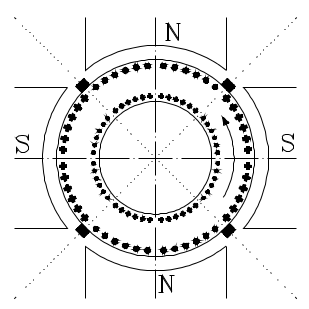
\includegraphics[scale=0.4]{ch4/image6.png}
		\captionof{figure}{ }
		\end{wrapfigure}
		La f.e.m. (tension à vide) d'une dynamo est $\propto$ au flux 
		utile par les pôles et la vitesse de rotation. Cette formule 
		reste valable pour une machine en charge ($i_a\neq0$) si on 
		considère que $\Phi$ pourrait être modifié par $i_a$. $\Phi$ 
		dépend de $i_e$ de façon non-linéaire (cf. labo).\\
		
		Ci-contre, la répartition des f.e.m. engendré pour une dynamo 
		à induit infiniment divisé de spires diamétrales. La tension 
		entre deux balais est la somme ($\int$) de toutes les f.e.m. 
		sous un même pôle. Ce schéma confirme que la f.e.m. est bien 
		alternative mais constante en un point fixe : 
		\textbf{pseudo-stationnaire} du à l'effet redresseur du 
		collecteur.

		\subsubsection{Méthode des circuits}
		\begin{wrapfigure}[10]{r}{2.8cm}
		\vspace{-5mm}
		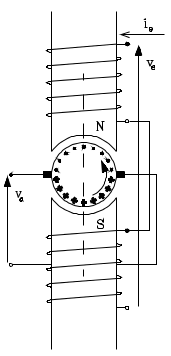
\includegraphics[scale=0.5]{ch4/image7.png}
		\captionof{figure}{ }
		\end{wrapfigure}
		Soit deux enroulements : un d'excitation parcouru par $i_e$ 
		et un induit pseudo-stationnaire à vide. A bornes du balais, 
		on a donc
		\begin{equation}
		v_a = R_ai_a+D\Psi_a
		\end{equation}
		où $\Psi_a$ est le flux coupé par l'enroulement induit, flux 
		créé par le courant d'excitation. On peut écrire
		\begin{equation}
		\Psi_a = M(\beta_m,i_e)i_e
		\end{equation}
		où $M$ est l'inductance mutuelle entre les enroulement $e$ 
		et $a$, mutuelle fonction de $\beta$, l'angle de décalage 
		entre $N$ et l'axe d'enroulement. En faisant les math ;
		\begin{equation}
		\begin{array}{ll}
		(v_a)_{i_a=0} &= \displaystyle D\Psi_a\\
		&= \displaystyle D(Mi_e)\\
		&= \displaystyle  DM\ i_e + M\ Di_e\\
		&= \displaystyle \frac{\partial M}{\partial \beta_m}D\beta_m
		i_e + \frac{\partial M}{\partial i_e}Di_e i_e + M\ Di_e\\
		&= \displaystyle G(\beta_m,i_e)\Sigma_r i_e +\left(M+\frac{
		\partial M}{\partial i_e}i_e\right)Di_e
		\end{array}
		\end{equation}
		On définit alors la valeur locale (ou différentielle) de la 
		mutuelle : $\displaystyle M' = M+\frac{\partial M}{\partial 
		i_e}i_e$, qui sera nulle si les balais sont calés sur l'axe 
		neutre ($\beta = \pi/2$) car $a \perp e$. \\
		On définit également la \textbf{fonction d'excitation}
		\begin{equation}
		G(i_e) = \frac{\partial M(\beta_m,i_e)}{\partial \beta_m}) =
		\frac{(\partial \Psi_a/\partial \beta_m)}{i_e}\qquad si\qquad 
		\beta=\frac{\pi}{2}, i_e=\text{ cste}
		\end{equation}
		La f.e.m. vaut alors $e = (v_a)_{i_a=0} = G(i_e)i_e\Omega_r$ 
		qui ressemble à notre belle formule encadré plus haut ! On 
		peut dès lors écrire
		\begin{equation}
		G(i_e)i_e = K\Phi
		\end{equation}
		La connaissance de la caractéristique à vide qui conduisait 
		immédiatement à la détermination de $K, \Phi$ en fonction de 
		$i_e$, il en est de même pour $G$ en fonction de $i_e$.
		
	\subsection{Effet de décalage des balais}
	\begin{wrapfigure}[7]{r}{9.5cm}
	\vspace{-8mm}
	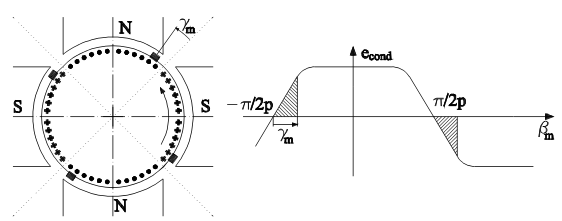
\includegraphics[scale=0.5]{ch4/image8.png}
	\captionof{figure}{ }
	\end{wrapfigure}
	Dans l'expression de la tension à vide, on a maintenant comme 
	limites $-\frac{\pi}{2}p+\gamma_m$ et $\frac{\pi}{2}p+\gamma_m$ (à 
	la place de $-\frac{\pi}{2}p+$ et $\frac{\pi}{2}p$), réduisant la 
	valeur de celle-ci par rapport à leurs positions sur les axes neutres. 
	Il faut encore rajouter à ça un effet de mutuelle.
	
	\subsection{Tension à vide - modèle mathématique}
	Trois remarques sur ce qu'est un bon modèle
	\begin{enumerate}
	\item Adapté au but poursuivi, ça ne sert à rien de faire trop.
	\item Il doit être simple, sinon avoues que tu ne le liras pas.
	\item Il doit être homogène, si on applique une hypothèse il faut 
	toujours l'appliquer.
	\end{enumerate}\ \\
	
	\textsc{Exemple - dynamo à vide}\\
	Définissions comme variables de commande $v_e$ la tension aux bornes 
	du circuit d'excitation, $\Omega_r$ la vitesse de rotation et $e$, 
	la tension à vides aux bornes des balais comme variable de sortie. 
	Connaissant deux expressions pour $e$, il suffit d'en prendre une et 
	de la compléter par l'équation du circuit d'excitation pour obtenir le 
	modèle recherché : $v_e = R_ei_e +D\Psi_e$.
	
		\subsubsection{Modèle non-linéaire}
		Il suffit d'utiliser une relation non-linéaire entre $\Psi_e$ 
		et $i_e$ pour compliquer le tout : $\Psi_e = L_e(i_e)i_e$ où 
		$L_e$ est l'inductance propre du circuit d'excitation, fonction 
		non-linéaire. Si l'on considère que $\Psi_e$ est variable d'état :
		ré-écrivons notre équation sous la forme d'une ED :
		\begin{equation}
		D\Psi_e = v_e-R_ei_e(\Psi_e)
		\end{equation}
		Si cette fois on choisi $i_e$ comme variable d'état, on peut 
		écrire
		\begin{equation}
		\dfrac{\partial \Psi_e}{\partial i_e}Di_e = v_e-R_ei_e\quad 
		\Longrightarrow\quad Di_e = \dfrac{v_e - R_ei_e}{L_e'}
		\end{equation}
		où $L_e'(i_e)$ est la valeur différentielle de l'inductance 
		propre du circuit $e$. Notons qu'elle est aussi égale à 
		$L_e+(\partial L_e/\partial i_e)i_e = \partial\psi_e/\partial 
		i_e$. Sachant que $e = (v_a)_{i_a=0} = G(i_e)i_e\Omega_r$, le 
		calcul de $e$ est immédiat si l'on a $i_e$.\\

		\begin{wrapfigure}[6]{l}{7cm}
		\vspace{-8mm}
		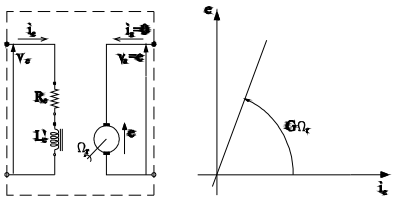
\includegraphics[scale=0.5]{ch4/image9.png}
		\captionof{figure}{ }
		\end{wrapfigure}
		Nos deux équations trop stylées 
		\begin{equation}
		\begin{array}{ll}
		v_e &= R_ei_e + L_e Di_e\\
		e &= K\Phi\Omega_r = G\Omega_ri_e
		\end{array}
		\end{equation}
		nous fournissent un schéma équivalent dont la caractéristique 
		permet le passage de $\Psi_e$ à $i_e$.
		
		Il est également possible, via $D\Psi_e = v_e - R_ei_e(\Psi_e)$ 
		d'obtenir le schéma-bloc suivant :
		\begin{center}
		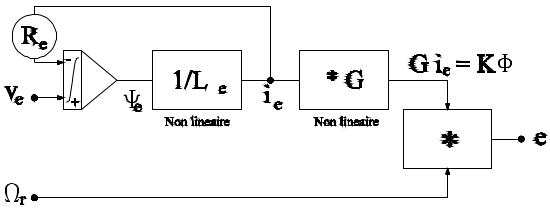
\includegraphics[scale=0.5]{ch4/image10.png}
		\captionof{figure}{ }		
		\end{center}			
		
		\subsubsection{Modèle linéaire}
		On peut l'obtenir en considérant de "petits mouvements" et en 
		substituant les courbes par leurs tangentes. Supposons que 
		$L_e = L_e' = L_{e,ns} = \text{cste}$ et $G = G_{ns} = 
		\text{cste}$. Notre précédente relation devient alors 
		\begin{equation}
		Di_e = \frac{v_e - R_ei_e}{L_e} \quad \lt\quad I_e(p) : 
		\frac{1}{1+pT_e}\frac{V_e(p)}{R_e}
		\end{equation}
		où $T_e = L_e/R_e$ est la constante de temps du circuit d'
		excitation (valeur assez élevée comme beaucoup d'enroulements). 
		Cette relation obtenue via Laplace est assez évidente à vue 
		du schéma équivalent, car ce-dernier est constitué de $R_e$ 
		et $L_e$. La grandeur de sortie vaut toujours 
		\begin{equation}
		e = Gi_e\Omega_r
		\end{equation}
		et dépend linéairement de $i_e$ si la vitesse est constante. 
		Le système global est du premier ordre
		\begin{equation}
		E(p) = G\Omega_r I_e(p) = G\Omega_r \dfrac{1}{1+pT_e}\frac{V_e
		}{R_e}
		\end{equation}
		\begin{center}
		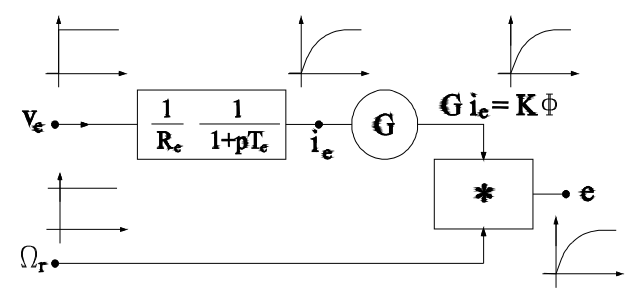
\includegraphics[scale=0.5]{ch4/image11.png}
		\captionof{figure}{ }		
		\end{center}			
		
			
\section{Influence du courant d'armature}
En effet, ça on sent que la machine en charge comportera en plus d'une 
source de tension une résistance $R_a$ et une inductance $L_a$.

	\subsection{Effet Joule (résistance $R_a$)}
	On les trouve dans l'enroulement ainsi que dans le ballais/collecteur,
	dépendant de plusieurs paramètres tel que la température et la valeur du courant.
	Mesurer la résistance globale n'est pas aisé, la résistance n'étant 
	pas la même quand la machine est en fonction ou non : en rotation, 
	elle est perturbée par la f.e.m. rémanente. En gros, les chutes sont 
	\begin{equation}
	\Delta V_{R_a} = \Delta V_b\text{sign}(i_a) + R_ai_a
	\end{equation}
	où $\Delta V_b$ représente la chute balais collecteur (fonction du 
	sens de rotation) et $R_a$ la résistance entre enroulements. Par 
	\textbf{convention}, la chute est fixée à $2V$ pour les balais en 
	carbone et $0.6V$ pour les métalliques.
	
	\subsection{Réaction transversale de l'armature infiniment divisée}
	\begin{wrapfigure}[9]{l}{4.7cm}
	\vspace{-5mm}
	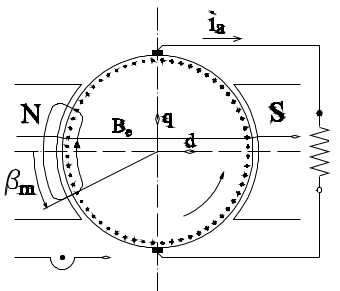
\includegraphics[scale=0.34]{ch4/image12.png}
	\captionof{figure}{ }
	\end{wrapfigure}
	Soit une génératrice avec un courant infiniment divisé qui circule 
	dans l'induit, même sens que la f.e.m. Les courants induits créent 
	à leurs tour un champ créant un flux perpendiculaire au flux 
	inducteur. En désignant $\beta_m$ l'abscisse angulaire d'un point, 
	calculons les ampères-tours dans un contour d'induction fermé :
	\begin{equation}
	\frac{N_c}{2\pi}\frac{i_a}{2d}2\beta_m
	\end{equation}
	Par symétrie par rapport à l'axe des pôles, la moitié des A.t. est 
	attribué à la moitié du chemin. Par abus, on attribue des A.t. la 
	ou le chemin traverse l'entrefer. Si ce dernier est constant et le 
	fer parfait 
	\begin{equation}
	H(\beta_m) = \frac{N_c}{2\pi}\frac{i_a}{2d}\frac{\beta_m}{\delta}
	\end{equation}
	$H$ est max si $\beta_m=\pi/2p$ : 
	\begin{equation}
	H\left(\frac{\pi}{2p}\right) = \frac{N_c}{2\pi}\frac{i_a}{2d}\frac{
	\pi}{2p\delta} = \frac{N_c}{8\delta}\frac{i_a}{pd}=\frac{N_s}{4\delta}
	\frac{i_a}{pd}
	\end{equation}
	Si le fer est réel il suffit de multiplier par $\mu_0$. Tout ceci 
	est bien indépendant de la vitesse de rotation : la situation est 
	la même que si une bobine était alignée sur l'axe neutre.
	
		\begin{center}
		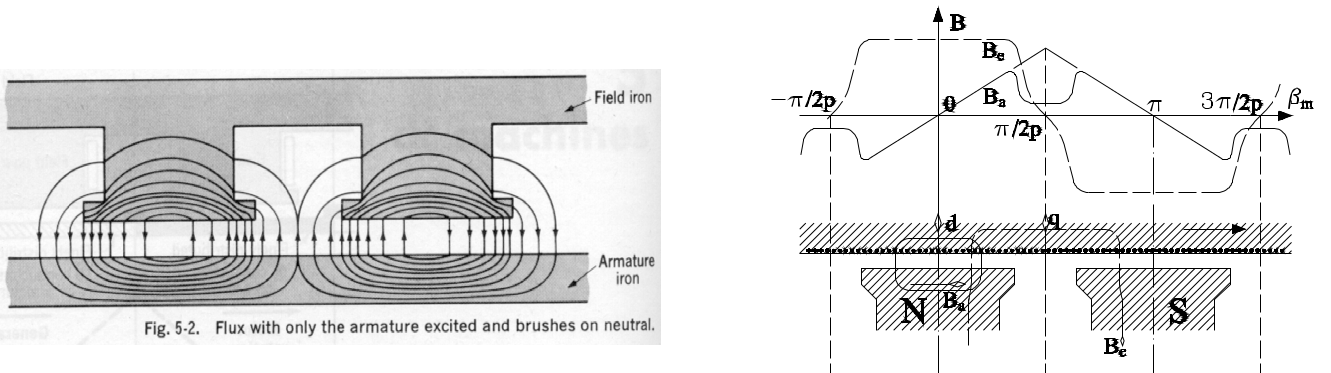
\includegraphics[scale=0.35]{ch4/image13.png}
		\captionof{figure}{ }		
		\end{center}
	
	Pour calculer $L_a$ on considère un enroulement fictif dont toutes 
	les spires ont par axe celui du balai : le flux vaudra l'intégrale 
	de l'induction entre $\beta_m et \pi-\beta_m$. Grâce au flux 
	totalisé : $L_a=\Psi_a/i_a$.
	
	\subsection{Le champ résultant}
		\subsubsection{Sans saturation}
		\begin{wrapfigure}[7]{r}{4.7cm}
	\vspace{-25mm}
	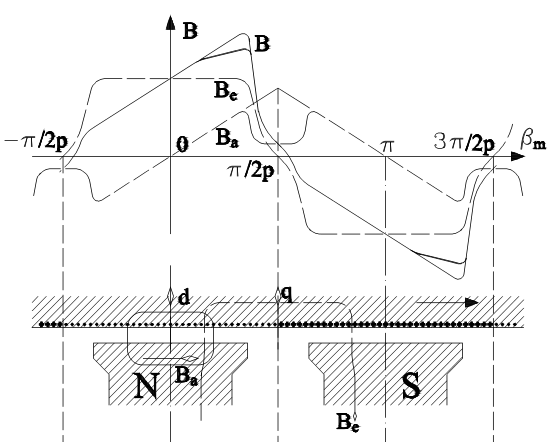
\includegraphics[scale=0.34]{ch4/image14.png}
	\captionof{figure}{ }
	\end{wrapfigure}
		On peut appliquer le principe de superposition. Pour une dynamo, 
		une fois la réaction d'induit est magnétisante (corne d'entrée) 
		et une fois démagnétisant (corde de sortie). La figure ci-contre 
		montre comment obtenir $B$ par la somme de l'induction de l'inducteur 
		$B_e$ et la réaction d'induit $B_a$.\\
		Notons que le flux par pôle n'a pas changé, la f.e.m. en charge est la 
		même qu'à vide. Cependant, l'induction est tantôt plus grande tantôt plus 
		faible par endroit, donc certaines spires supportent plus de tensions et il y a 
		risque de claquage entre les lames du collecteur. 
		
		\subsubsection{Avec saturation}
		L'induction en charge est plus petite que la somme de l'excitation 
		et la réaction d'induit. Le flux longitudinal est plus faible, 
		causant une f.e.m. plus faible $\rightarrow$\textit{ La réaction 
		d'induit possède une composante longitudinale à cause de la 
		saturation.}. Pour décrire l'effet démagnétisant, trois hypothèses :
		\begin{enumerate}
		\item Lignes de forces radiales dans l'entrefer.
		\item L'induction null en dehors des pôles.
		\item Démonstration faite pour $p=d=1$.
		\end{enumerate}
		A vide, juste avec le courant d'excitation $i_e$ on a $A.t._e = 
		N_ei_e$. Si la spire n'est pas sous le pôle sa tension est nulle. 
		Si par contre elle est sous le pôle elle sera $\propto B_e$. La 
		courbe a vide donne le lien entre $e$ et $N_ei_e$ mais aussi la 
		f.e.m. à une constante près.\\
		Les courants induits causent également des A.t. de réactions 
		d'induits qui varient linéairement entre la corne de sortie $-A$ 
		et d'entrée $+A$ de la sorte :
		\begin{equation}
		A = \frac{N_c}{2\pi}\frac{i_a}{2}\frac{b_i}{4\pi R}
		\end{equation}
		Les A.t. varient ainsi linéairement de $N_ei_e-A$ à $N_ei_e+A$ (
		$OP_1$ à $OP_2$ sur le schéma page 4.33). \textbf{Lire le texte 
		sur cette page, c'est assez confus. Enes confirme.}
		
		\subsection{Couple électromécanique - Couple extérieur}
		La loi de Laplace ($F+ilB$) permet de calculer la somme sur 
		chaque conducteur pour ensuite les sommer, mais il est plus 
		simple d'utiliser la conservation de la puissance : la somme 
		de la puissance appliquée électriquement et de la puissance 
		appliquée mécaniquement est nulle\footnote{? (en convention 
		récepteur)} :
		\begin{equation}
		[\underbrace{P_{electrique} - (P_{pJoule}}_{P_{electromecanique}}
		+P_{pmagn})] + [P_{mecan}-P_{meca}]=0
		\end{equation}
		où les pertes joules $P_{pJ}=0$ si $î_a=0$. Par contre les pertes 
		magnétiques existent tout de même (hystérèse, Foucault, ...). Les 
		pertes méca sont dues aux frottement (fonction de $\Omega_r$). La 
		puissance mécanique appliquée à un moteur est négative. On peut 
		calculer le couple électromécanique $P_{em} = C_{em}\Omega_r$. D'autre part,
		\begin{equation}
		\begin{aligned}
			P_{em} &= P_{électrique} - P_{pJ}\\
						 &= v_a i_a - \Delta V_b i_a -R_a i_a^2\\
						 &= e i_a
		\end{aligned}
		\end{equation}
		En utilisant \autoref{eq:4.5}, on trouve que 
		\begin{equation}
			C_{em} = K\Phi i_a = Gi_ei_a.
		\end{equation}
		En moteur, la réaction d'induit change de signe : magnétisante sous la corne polaire d'entrée.\\
		
		\textbf{Réécriture de Nicolas Englebert}
		
	\subsection{Inconvénients de la réaction d'induit}
	Cette réaction cause trois effets néfastes :
	\begin{enumerate}
	\item Déplacement de la ligne neutre ($B=0$) gênant la commutation
	\item Augmente l'indiction : risque de claquage entre les lames
	\item Cause de l'inductance du rotor, s’opposant aux variations rapides 
	du courant induit et donc du couple
	\end{enumerate}
	
	
	\subsection{La commutation}
	La commutation concerne tous les phénomènes inversant le signe du courant 
	par court-circuit/circuit ouvert avec les balais. Comme il y a frottement, 
	il peut y avoir étincelles !
	
	\begin{description}
	\item[Causes mécaniques] Certaines lames bombées, vibrations, mauvais 
	équilibrage, \dots
	\item[Causes électriques] Théoriquement très compliqué
	\end{description}
	Détaillons légèrement ce point \textit{compliqué} avec la théorie de ARNOLD. 
	On se débarasse d'abord de toute imperfections mécaniques en trois hypothèses :
	état mécanique parfait, résistivité balais/collecteur constante, égalité de 
	la largeur d'un balai et d'une lame.\\
	
	Le souci est inductif. Au moment de la commutation, l'inductance à tendance 
	à ne pas laisser passer le courant. Plus mathématiquement, à cet instant la 
	dérivée du courant subit une discontinuité causant une surtension importante : 
	rupture de l’isolation et risque de claquage.\\
	
	Au cours oral, le prof a dit qu'il ne poserait pas de question de démonstration sur cette partie. Lire et comprendre le phénomène au travers les équations peut s'avérer utile. \\
	
	\textsc{Le remède de grand-mère}.\\
	L'idée est de créer un phénomène d'amplitude 
	contraire et même encore plus fort (pour être sûr) pour contrecarrer cet 
	effet. On crée alors une fem opposée, favorable à la variation de courant afin 
	de permettre la variation de courant en fin de commutation. On crée cette fem 
	grâce a un flux d'axe neutre (transversal) au sens opposé à la réaction d'induit. On a dès lors l'intégration de pôles de commutation avec des enroulements de compensation. \\
	On pourrait aussi se dire \textit{"Pourquoi ne pas prendre un entrefer plus grand?"} 
	Effectivement, l'inductance diminue mais le flux d'excitation également ce qui 
	est moins avantageux. 
		

\section{Étude de la dynamique des machines}
	\subsection{Modèles mathématiques - schémas équivalents}
		\begin{wrapfigure}[10]{l}{8.7cm}
	%\vspace{-25mm}
	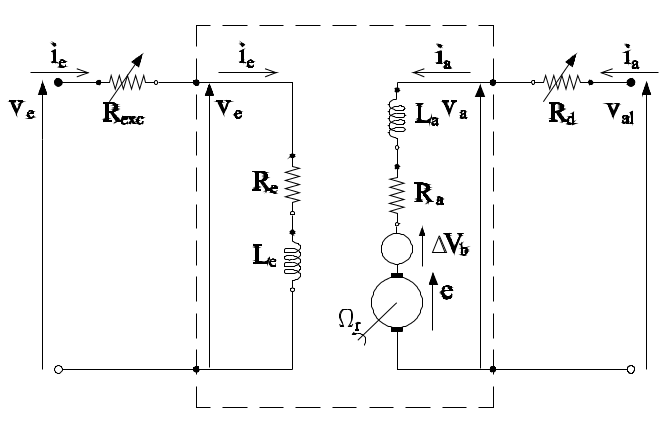
\includegraphics[scale=0.34]{ch4/image15.png}
	\captionof{figure}{ }
	\end{wrapfigure}
	Reprenons ce qui a été vu précédemment et synthétisons le sur le schéma ci-contre. 
	On va supposer que le modèle magnétique, les pertes, \dots sont linéaires. On 
	trouve 
	\begin{description}
	\item[$R_e$;] Résistance du circuit inducteur
	\item[$L_e$;] Inductance du circuit inducteur
	\item[$R_a$;] Résistance du circuit d'induit
	\item[$\Delta V_b$;] Chute de tension du contact balais-collecteur
	\item[$L_a$;] Inductance du circuit d'induit
	\item[$e$;] Force électromotrice engendrée $= Gi_e\Omega_r$
\end{description}		
	Notre tension d'excitation $V_e$ pourra être éventuellement réglable : $V_x$. La 
	zone en pointillé représente la machine, tandis que la partie de droite représente 
	le rotor, possédant une fem $e$ du à sa rotation.\\
	
	Lors de l'allumage, il faut fournir énormément de flux. Pour limiter ce courant, on 
	introduit des réhostas :
	\begin{description}
	\item[$R_d$ : rhéostat de démarrage;]  Sert à limiter le courant à la mise sous tension 
	$V_{al}$ car à vitesse nulle, $e=0$ et le courant est juste limité par $R_a$ et $L_a$ 
	de faible valeur.
	\item[$R_{exc}$ : rhéostat d'excitation;] Règle le courant d'excitation $i_e$ pour une 
	tension d'excitation $v_x$ donnée.
	\end{description}
	Les équations de ce modèles sont, pour rappel :
	\begin{equation}
	\begin{array}{ll}
	v_x &= (R_e+R_{exc}-i_e + L_e\frac{di_e}{dt}\\
	v_{al} &= e+\Delta V_b + (R_a+R_d)i_a + L_a\frac{di_a}{dt}\\
	e &= k\phi\Omega_r = Gi_e\Omega_r
	\end{array}
	\end{equation}
	Cette fois-ci, on doit ajouter l'équation de mouvement :
	\begin{equation}
	j\dfrac{d\Omega_r}{dt} = C_{em}+C_r
	\end{equation}
	avec $C_r$, le couple résistant du moteur (pertes magnétiques et mécanique). 
	Il doit être vu comme négatif, diminuant le couple appliqué par le moteur à l'arbre, 
	$C_{em}$.\\
	Il s'agit d'un modèle dynamique (dérivée). En laboratoire, tout peut être mis comme 
	étant constant. Sous la forme canonique, on obtient :
	\begin{equation}
	\begin{array}{ll}
	Di_e &= \frac{1}{L_e}[v_x-(R_e+R_{exc}i_e]\\
	Di_a &= \frac{1}{L_a}[v_{al} - \Delta V_b - Gi_e\Omega_r - (R_a+R_d)i_a]\\
	D\Omega_r &= \frac{1}{J}[Gi_ei_a - C_r(\Omega_r)]
	\end{array}
	\end{equation}
	Avec ces équations, il est facile d'obtenir le schéma bloc ci-dessous.  
	\begin{itemize}
	\item[$\bullet$] Notre sortie est bien la vitesse de rotation, définie par le couple 
	moteur.
	\item[$\bullet$] La première équation est représenté à gauche sur la branche $V_x$ : 
	on calcule $i_e$ à partir de $V_x$.
	\item[$\bullet$] La grandeur d'entrée de la deuxième équation est la tension d'alimentation. 
	Il faut ainsi partir de $V_{al}$, soustraire $Gi_e\Omega_r,\dots$. Le $Gi_e$ avait déjà été 
	calculé, $\Omega_r$ est à la sortie. Le rectangle central correspond ainsi à une partie de 
	cette deuxième équation
	\item[$\bullet$] Pour la troisième équation, nous avons $K\phi i_a$ et il faut rentrer 
	le couple résistant : on peut dire que le couple résistant dépend de la vitesse de 
	rotation
	\end{itemize}
	
	\begin{center}
	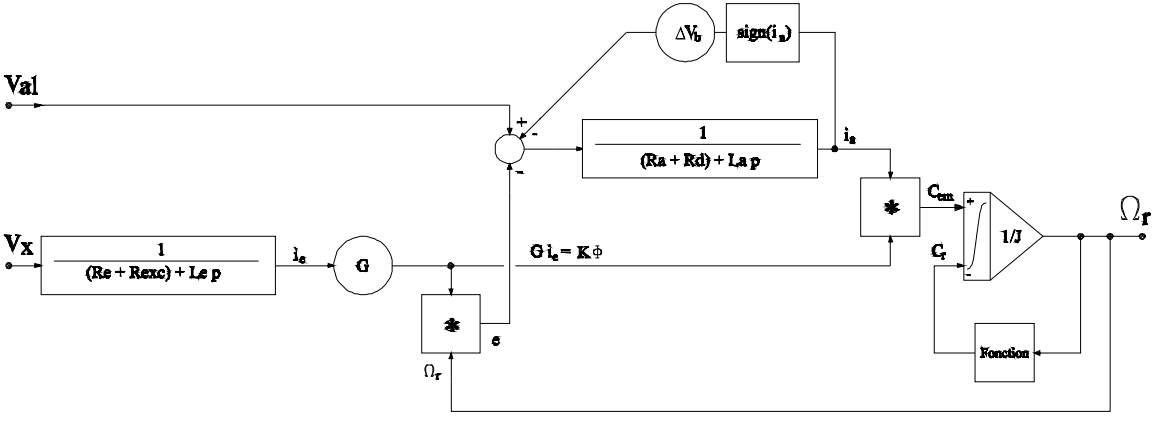
\includegraphics[scale=0.34]{ch4/image21.png}
	\captionof{figure}{ }
	\end{center}
	
	Supprimons la dernière rétroaction. Mettons notre pied sur l'intégrale pour avoir un couple 
	constant. Le couple moteur étant constant, la vitesse ne change pas directement (du à la grande 
	inertie)(nous 
	étions en situation de régime, on vient de briser cet équilibre). Mais maintenant, on sait que 
	la vitesse va diminuer. Sachant cela,  le carré avec (*) au milieu va être affecté. Comme 
	$i_e$ est contant, la fem $e$ va diminuer : déséquilibre le rond avec $\pm$.\\
	
	A l'examen oral, je peux négliger le bras tout en haut en affirmant que c'est un effet 
	correcteur pas très important, que l'ordinateur peut se charger de le calculer.\\
	
	Ceci étant dit, La valeur $V-e$ va commencer à être positive, le courant va alors 
	augmenter. Le couple moteur va alors lui aussi augmenter pour retrouver le couple appliqué 
	par mon pied et on retrouvera un nouveau point d'équilibre, avec une vitesse plus faible 
	mais un courant plus important (car couple plus important).\\
	
	Si la vitesse diminue de 1\%, la vitesse fait-elle de même ? Le courant augmentera en 
	réalité plus rapidement que cette diminution. Pour savoir à quel point, il faut annuler 
	toutes les dérivée pour se rendre compte que le terme $1/R_a$ est très important : le couple 
	va vite réagir à une petite variation.\\
	
	En faisant une analyse semblable, on peut voir que si on augmente $V_x$, le moteur va 
	tourner moins vite. L'augmentation de $V_d$ cause par contre une augmentation de la 
	vitesse.
	
	
\section{Courbes caractéristiques des génératrices}
	
	\subsection{Les différents types de génératrices}
	\begin{wrapfigure}[7]{l}{3cm}
	\vspace{-5mm}
	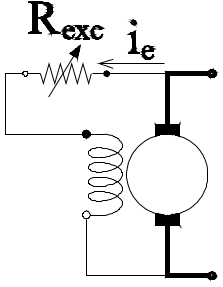
\includegraphics[scale=0.34]{ch4/image16.png}
	\captionof{figure}{ }
	\end{wrapfigure}
	On a toujours considéré que le courant d'excitation était fourni par une source 
	extérieure. Or, à cause du rémanent, une tension existe lors de la rotation entre 
	les balais de la machine pour un courant d'excitation nul. L'idée est d'utiliser 
	ce courant pour exciter la machine\footnote{Oh oui elle est chaude !}.\\
	S'il n'y a pas de charge, $i_e$ est très petit et on considère que la tension aux 
	bornes est la fem. Pour $\Omega_r$ donné, on a deux caractéristiques :
	\begin{enumerate}
	\item Caractéristique à vide $e = f(i_e)$.
	\item Loi d'Ohm du circuit d’excitation $e=(R_{exc}+R_e)i_e$.\footnote{En régime, 
	il n'y a que les résistances : la self se comporte comme un fil.}
	\end{enumerate}
	\begin{center}
	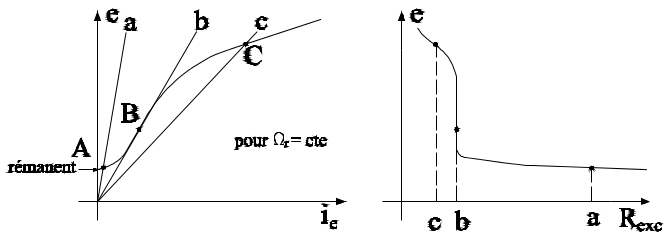
\includegraphics[scale=0.37]{ch4/image17.png}
	\captionof{figure}{ }
	\end{center}
	L'intersection donne le point de fonctionnement. On voit qu'il existe une valeur 
	de $R_{exc}$ au dela de laquelle la tension aux bornes est très faible (a). Si 
	on inverse les bornes, la machine ne s'amorce pas et si la machine est linéaire, 
	le seul point de fonctionnement est $e=0,i_e=0$ sauf si $R_{exc}+R_e=G\Omega_r$.\\
	
	En pratique, on rencontre trois types de génératrices :
	\begin{description}
	\item[Excitation dirigée / shunt] Beaucoup de spires pour avoir beaucoup 
	d'ampères-tours avec peu de flux
	\item[Excitation série] Ce type de moteur est caractérisé par le fait que 
	le stator (inducteur) est raccordé en série avec le rotor (induit) : le même 
	courant traverse le rotor et le stator. Cela offre une faible résistance, et 
	le nombre de spire nécessaire est moins important ($\approx 100$ fois moins qu'en 
	shunt).\footnote{ On fait tourner le moteur : entre les balais on obtient $e$. Pour avoir 
	le flux, on passe tout le courant dans l'excitation.}
	\item[Compoundage] Les deux en même temps.
	\end{description}
	
	
	\subsection{Caractéristiques à vide et en charge d'une machine à excitation 
	indépendante}
		\subsubsection{Fem à vide}
			\begin{wrapfigure}[7]{r}{3.3cm}
	\vspace{-5mm}
	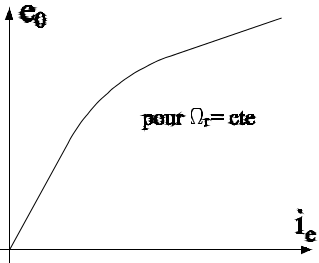
\includegraphics[scale=0.34]{ch4/image18.png}
	\captionof{figure}{ }
	\end{wrapfigure}
		Négligeons l'hystérèse. Ici on place le voltmètre sur les balais pour mesurer 
		la fem à vide. Le courant $i_e$ comprend le rhéostat et le rémanent n'est 
		pas représenter. Initialement la courbe est "droite" puis on arrive à saturation.
		
		
		\subsubsection{Fem et tension en charge}
		La tension aux bornes de la machine est donnée par (courant de charge fixé) :
		\begin{equation}
		v_a = e - R_ai_a - \Delta V_b
		\end{equation}
		où $e$ vaut la fem à vide correspondant à $i_e' = i_e-i_{eri}$ où $i_{eri}$ 
		est le courant d’excitation correspondant aux A.t. démagnétisant de la réaction 
		d'induit.\\
		\danger Si le flux est perpendiculaire, cela n'influe pas sur d'autres flux.\\

		\begin{center}
		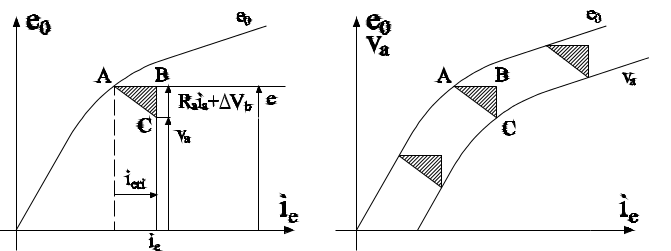
\includegraphics[scale=0.43]{ch4/image19.png}
		\captionof{figure}{ }
		\end{center}		
		
		\begin{wrapfigure}[9]{l}{3.3cm}
		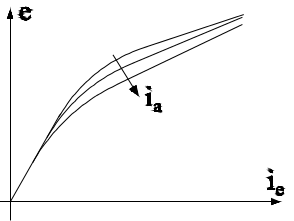
\includegraphics[scale=0.34]{ch4/image20.png}
		\captionof{figure}{ }
		\end{wrapfigure}
		On déduit le caractéristique en charge de celle à vide en décalant chaque 
		point du triangle des pertes $ABC$ où $AB$ vaut $i_{eri}$ et $BC$ vaut 
		$R_ai_a + \Delta V_b$. En supposant que pour $i_a$ fixé, $R_a/i_{eri} =\ cste$, 
		on déduit la caractéristique en charge par translation $AC$.\\
				
		En pratique, $i_{eri} =\ cste$ si $i_a =\ cste$ n'est vérifiée que pour un 
		petit domaine, les courbes ne sont pas des parfaites translation. On remarque 
		sur la courbe réelle, qu'au début, il n'y a pas de réaction d'induit. Ces 
		courbes sont également commune "à la fin" à cause de la saturation.
		
		
\section{Courbes caractéristiques des moteurs}
On cherche à caractériser le courant consommé par le moteur, $i_a$ et $-C$ le couple 
net appliqué à la charge tel que
\begin{equation}
-C = C_{em} - C_{pmeca} - C_{pmagn}
\end{equation}
		
	\subsection{Caractéristique à vide en moteur $\Omega_r = f(i_e)$}
	Supposons $V_{al}$ constante, $R_d=0$ (en régime), $R_a$ constante (pas d'effet 
	thermique) et négligeons $\Delta V_b$. On suppose que la caractéristique à vide,
	en génératrice, 	prise à la vitesse de référence $\Omega_g$ est connue :
	\begin{equation}
	e_{0g} = f(i_e)
	\end{equation}
	Mais aussi la famille des courbe des f.e.m. en charge :
	\begin{equation}
	e_g = f(i_e,i_a)\qquad \forall i_a
	\end{equation}
	La caractéristique à vide du moteur lie $\Omega_r = f(i_e)$ pour $V_a=\ cste$ et 
	couple moteur nul. Le couple EM sert alors juste à compenser les pertes mécaniques : 
	courant absorbé très faible\footnote{Car le moteur n'entraîne rien}, tension aux 
	bornes $\approx$ fem à vide :
	\begin{equation}
	v_a = e+R_ai_a + \Delta V_B \approx e \approx e_0
	\end{equation}
	On on sait que (en moteur) $\displaystyle e_0 = K\Phi(i_e)\Omega_r \Longrightarrow 
	\Omega_r = 	\dfrac{e_0}{K\Phi(i_e)}$. Pour la même valeur du courant d’excitation, 
	la caractéristique à vide (en génératrice) donne $e_{0g} = K\Phi(i_e)\Omega_g$. On a donc :
	\begin{equation}
	\Omega_r = 	\dfrac{e_0}{K\Phi(i_e)}\ \ \text{ feat. }\ \ \left\{\begin{array}{ll}
	v_a &\approx e_0\\
	\frac{1}{K\Phi(i_e)} &= \frac{\Omega_g}{e_{0g}(i_e)}
	\end{array}\right.\quad  \Longrightarrow\quad \Omega_r = \Omega_g\dfrac{v_a}{e_{0g}(i_e)}
	\end{equation}
	
	\begin{wrapfigure}[9]{l}{5.3cm}
	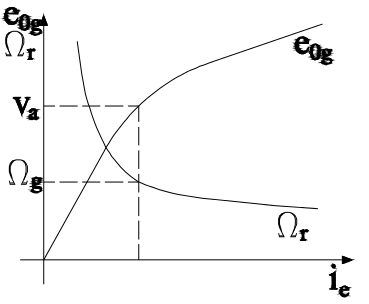
\includegraphics[scale=0.34]{ch4/image22.png}
	\captionof{figure}{ }
	\end{wrapfigure}
	On remarque que la caractéristique à vide en moteur est, à une constante près, 
	l'inverse de celle en génératrice. On voit que la vitesse \textbf{diminue} quand 
	$i_e$ \textbf{augmente}\footnote{Comme vu précédemment sur le schéma bloc à cause 
	de la rétroaction!} Il faut démarrer le moteur à pleine excitation ($i_e=i_{max}$) 
	pour avoir le couple moteur maximal. On voit également que si on diminue trop 
	l'excitation (coupe un fil) la vitesse augmente : danger mécanique $\rightarrow$ le 
	courant n'est plus limité que par la résistance d'induit et peut atteindre dix 
	fois le courant nominal. Les disjoncteurs se chargent de protéger la machine.
	
	
	\subsection{Caractéristiques en charge - moteur à excitation indépendante}
	On peut voir le "en charge" comme un freinage, charge dont le couple résistif est 
	connu. La puissance mécanique va changer et il y aura des effets sur la vitesse et 
	la consommation (le courant d'alimentation change même si la tension d'alimentation 
	est constante).\\
	On suppose que $i_e=\ cste$ et $v_a =\ cste = V_{al}$. On sait que :\\
	
	\retenir{\begin{equation}
	\begin{array}{ll}
	v_a &= e+ \Delta V_b + R_ai_a\\
	e &= K\Phi\Omega_r\\
	C_{em} &= K\Phi i_a\\
	-C &= C_{em} - C_p\\
	e_g &= f(i_e,i_a)\quad \text{à $\Omega_g$ donné)}\\
	K\Phi &= \frac{e}{\Omega_r} = \frac{e_g}{\Omega_g}
	\end{array}
	\end{equation}
	avec $C_p$ le couple des pertes (frottement, Foucault, \dots). L'ensemble des 
	courbes mesurées en génératrice est donnée par $e_g$. Comme le flux est difficile 
	à mesurer, 	on le calculera via $e_g/\Omega_g$ avec $\Delta V_b$ négligé (dernière 
	équation). Notons qu'il n'y a ici pas de dérivée : nous sommes en régime.}\ 
	
	Nous avons donc
	\begin{equation}
	\begin{array}{ll}
	\Omega_r &= \dfrac{e}{K\Phi}\\
	&= \dfrac{v_a -\Delta V_b\text{sign}(i_a) - R_ai_a}{e_g/\Omega_g}\\
	&= \Omega_g\dfrac{v_a -\Delta V_b - R_ai_a}{e_g}	
	\end{array}
	\end{equation}
	
		\subsubsection{a. $\Omega_r = f(i_a)$}
		Supposons la réaction d'induit négligeable : $e_g(i_e,i_a) = e_{0g}(i_e)$. D'où
		\begin{equation}
		\Omega_r = \Omega_g \dfrac{v_a-\Delta V_b\text{ sign}(i_a)}{e_{0g}(i_e)}- 
		\Omega_g \dfrac{R_ai_a}{e_{0g}(i_e)}
		\end{equation}

\begin{center}
	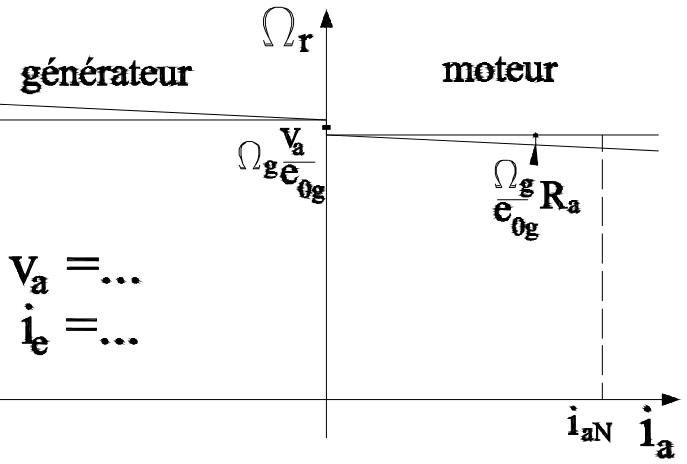
\includegraphics[scale=0.34]{ch4/image23.png}
	\captionof{figure}{ }
\end{center}
		Comme $R_a$ est très petit, notre terme sera presque une droite horizontale : à 
		$V_a, i_e=\ cste$, la vitesse de rotation à excitation indépendante dépend peu de 
		la charge. C'est rassurant, car nous avions vu que la vitesse n'allait que peu 
		changer quand on dépose son pied ! Le 	"saut" à l'intersection avec l'ordonnée 
		correspond à la variation de signe au niveau des balais. \\
		Quand on augmente $i_e$, $e_{0g}$ augmente aussi\footnote{Nos fameuses courbes $e_0$ 
		en fonction de $i_e$ (sans tenir compte de $i_a$ ici.} et la vitesse à vide diminue : 
		déplacement caractéristique (idem si $V_a$ diminue). \\
		
		Avec une réaction d'induit, pour $i_e$ fixé, la fem en charge $e_g$ diminue quand 
		$i_a$ augmente : augmentation de la vitesse de rotation en moteur aux valeurs 
		élevée du courant.
		\begin{center}
			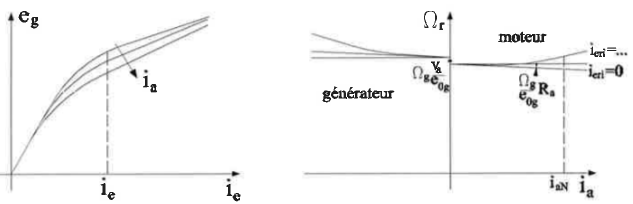
\includegraphics[scale=0.5]{ch4/image24.png}
	\captionof{figure}{Pour l'oral, ceci est un bon complément au schéma bloc vu plut haut! 
	Donne une explication plus matheuse.}
		\end{center}
	
		\subsubsection{b. $-C = f(i_a)$}
		Dans ce cas-ci on a : 
		\begin{equation}
		C_{em} = K\Phi i_a = \dfrac{g(i_e,i_a)}{\Omega_g}i_a
		\end{equation}
		avec $-C = C_{em}-C_p$. Attention, $C_{em}$ n'est pas le couple mécanique net utile ! 
		Pour $e_g(i_e,i_a)$ on utilise la courbe en génératrice et $\Omega_g$ est constante 
		en génératrice. \\
		Si la réaction d'induit est négligeable avec $i_e$ constant et $e_g=e_{0g}$ constant, 
		$C_{em}$ est linéaire en fonction du courant absorbé $i_a$. Comme la vitesse ne varie 
		que peu, il en est de même pour le couple de perte : le couple moteur est aussi linéaire 
		en fonction de $i_a$.
	

	
	
	
	
	
	
	
	
	
	
	
	
	
	
	
	
	
	
	
	
	
	
	
	
	
	
	
	
	
	
	
	
	
		
		
